% -----------------------------------------------------------------------------
% Fundamentação Teórica
% -----------------------------------------------------------------------------

\chapter{Fundamentação Teórica}
\label{chap:fundamentacaoTeorica}

Os protocolos, anteriormente mencionados neste trabalho, são um conjunto de formalidades a serem seguidas para permitir a conversação e o entendimento entre dois hosts. Nos modelos de conexão a serem apresentados (OSI e TCP/IP), estes protocolos são divididos em diferentes camadas para que assim os problemas a serem tratados também sejam divididos. Essa divisão se faz necessária devido à complexidade na comunicação. Além disso, este modelo provê a abstração de uma camada à respectiva camada superior.

Quando o dado é enviado de um host para outro, ele passa pelas várias camadas estruturadas ainda no remetente, as quais adicionam informações ao dado, que serão necessários para seu entendimento ou envio, encapsulando-o, gerando assim uma nova PDU (\textit{Protocol data unit}) a cada camada. Ao chegar no host destino este dado passa novamente pela pilha, porém em sentido inverso, e cada camada retira e interpreta o pacote enviado pela camada correspondente e repassa o pacote resultante para camada superior. Este funcionamento pode é mostrado na Figura \ref{fig:camadas}, onde as PDU's são representadas pelos elementos ao lado de cada camada, é possível perceber seu incremento e decremento no host remetente e no host destino, respectivamente. Tudo isso é feito por protocolos pertencentes à cada nível, desta forma uma camada apenas conversa diretamente com sua correspondente.

\begin{figure}[H]
	\centering
    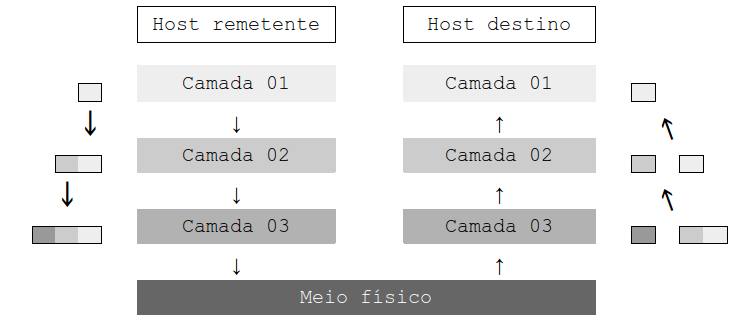
\includegraphics[width=\textwidth]{04-figuras/camadas.png}
    \caption{Funcionamento em camadas}
    \label{fig:camadas}
\end{figure}  	 
	 
	 
\section{Modelo de Referencia ISO OSI}

O modelo OSI (\textit{Open System Interconection}), Figura \ref{fig:OSI}, criado no final dos anos 70 pela ISO (\textit{International Standards Organization}), é um modelo conceitual estruturado em camadas, que de acordo com \citeonline{FOR} aborda todos os aspectos da comunicação de rede. Este mesmo autor define o termo "Sistema Aberto", contido em sua definição, como um conjunto de protocolos os quais permitem a comunicação entre dois sistemas distintos, inclusive em suas arquiteturas. 

\begin{figure}[H]
	\centering
    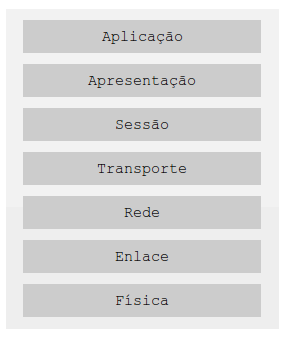
\includegraphics[width=0.5\textwidth]{04-figuras/OSI.png}
    \caption{Pilha do modelo de referência OSI}
    \fonte{\cite{COMER}}
    \label{fig:OSI}
\end{figure} 


Para que isto seja possível são necessárias camadas bem delimitadas e com fuç\~oes bem especificas: de acordo com \citeonline{STALLINGS}, limites bem definidos tornam possível que mudanças em uma camada não afetem os softwares existentes em outras camadas, já as restrições de suas funções provê o desenvolvimento independente de padrões.

\citeonline{COMER} ressalta ainda que este modelo foi criado para descrever protocolos em uma única rede, assim diferentemente do modelo TCP/IP, não contem uma camada específica para encaminhamento de internet.



\section{Modelo TCP/IP}

A arquitetura do modelo TCP/IP é apresentada no RFC 1122 \cite{RFC1122}, o qual especifica os requerimentos exigidos para que um host seja capaz de se conectar à Internet. Este explana sobre as três últimas camadas do modelo: transporte, internet e enlace; já a primeira camada é apresentada separadamente pelo RFC 1123 \cite{RFC1123}.

Diferentemente do modelo ISO o conjunto de protocolos TCP/IP não são necessariamente interdependentes. Segundo \citeonline{FOR}, os protocolos presentes nesse modelo possuem uma certa independência e podem ser organizados de acordo com a necessidade da rede. O termo hierárquico apenas garante que um protocolo da camada superior seja suportado por outro(s) protocolo(s) da camada inferior.

\begin{figure}[H]
	\centering
    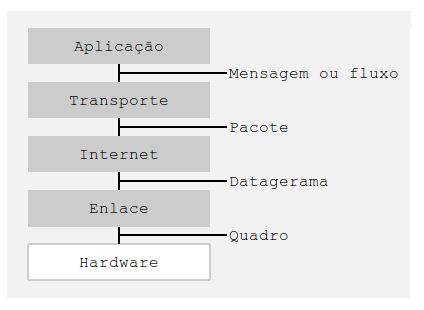
\includegraphics[width=0.65\textwidth]{04-figuras/TCPIP.png}
    \caption{Pilha do modelo TCP/IP e o nome das PDU's transferidas entre as camadas}
    \fonte{\cite{COMER}}
    \label{fig:TCPIP}
\end{figure} 

A Figura \ref{fig:TCPIP} representa a pilha do modelo TCP/IP e a nomenclatura referente aos pacotes, PDU's, transferidos entre cada camada. Já na Figura \ref{fig:relacao}, retirada do livro de \citeonline{FOR}, está representada a relação do modelo de camadas ISO e os protocolos pertencentes ao modelo TCP/IP. 

\begin{figure}[H]
	\centering
    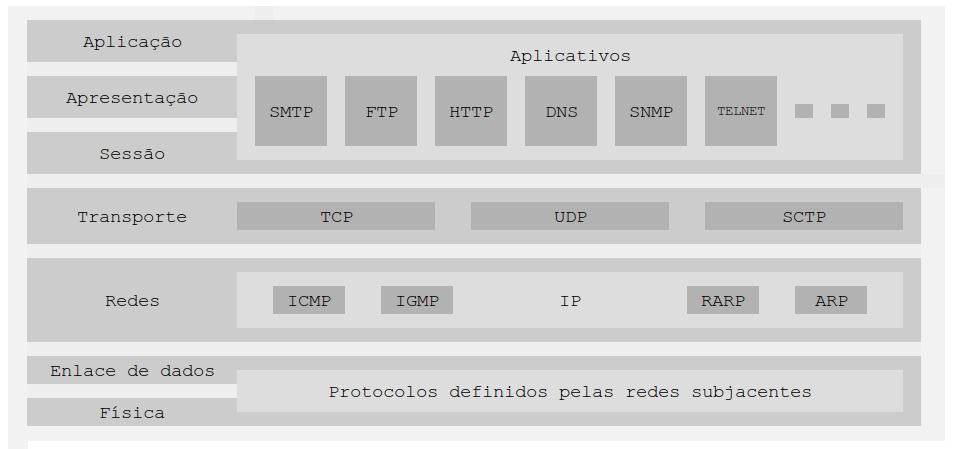
\includegraphics[width=\textwidth]{04-figuras/relacao.png}
    \caption{Relação entre o modelo de referência OSI e os protocolos pertencentes ao modelo TCP/IP }
    \label{fig:relacao}
    \fonte{\cite{FOR}}
\end{figure}    


Ademais é importante ressaltar que a maioria das literaturas que tratam deste assunto utilizam um modelo híbrido, entre o OSI e com TCP/IP. Este modelo apresenta 5 camadas e sua relação com o modelo original TCP/IP e o modelo OSI pode ser vista na Figura \ref{fig:tresmodelos}. De acordo com \cite{TANENBAUM} esse modelo visa incluir os benefícios de ambas referências. Enquanto a separaç\~ao do modelo OSI e as definições caracter\'isticas de suas camadas ainda o torna desej\'avel como referência, o modelo TCP/IP contribui com seus protocolos amplamente aplicados.

\begin{figure}[H]
	\centering
    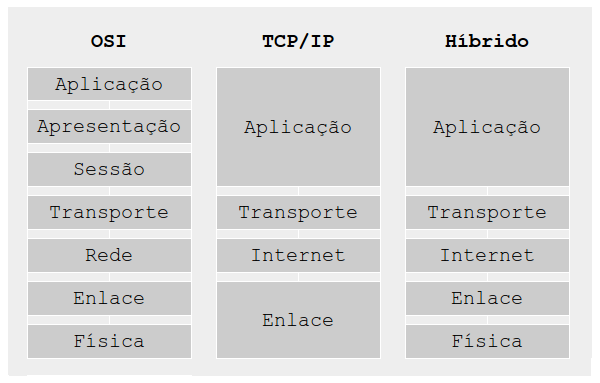
\includegraphics[width=0.75\textwidth]{04-figuras/tresmodelos.png}
    \caption{Relação entre o modelo de referencia OSI, o modelo de protocolos TCP/IP e o modelo híbrido}
    \label{fig:tresmodelos}
\end{figure} 

Neste trabalho iremos focar no modelo TCP/IP oficial, de quatro camadas, e seus protocolos, os quais serão apresentados nas subseções seguintes: 2.2.1 Aplicação, 2.2.2 Transporte, 2.2.3 Internet e 2.2.4 Enlace. 

\subsection{Aplicação}

A primeira camada da pilha TCP/IP é a de Aplicação, definida separadamente no RFC 1123 \cite{RFC1123}. Ela mantém protocolos necessários e utilizados pelos usuários e serviços. Em suma, aplicações de redes executadas em um sistema final tem o objetivo de se comunicar com outras aplicações  em outro host \cite{KUROSE}.

Os principais protocolos pertencentes à Aplicação, apresentados por \cite{STALLINGS}, são:
\begin{itemize}
\item Telnet: possibilita o usu\'ario acessar uma m\'aquina, atrav\'es de outro sistema.
\item FTP (\textit{File Transfer Protocol}): utilizado para transferir arquivos entre sistemas.
\item SMTP (\textit{Simple Mail Transfer Protocol}): prov\^e transporte de emails entre diferentes hosts.
\item HTTP (\textit{HyperText Transfer Protocol}): utilizado para a comunicação entre um sistema final e um servidor Web.
\item DNS (\textit{Domain Name System}): serviço de diretório que traduz nomes de hospedeiro para endereço IP.
\end{itemize}

Além de seus serviços é importante destacar as arquiteturas da camada de Aplicação. \citeonline{KUROSE} apresenta duas arquiteturas, as quais afirmam serem as mais comumente utilizadas hoje em dia, a cliente/servidor e a P2P(\textit{Peer to Peer}).

O autor explica que a arquitetura cliente/servidor é configurada em um sistema final, que atua como servidor (oferece serviço através de uma rede), este será acessado por um ou mais host(s), denominado(s) cliente(s) que enviam uma requisição ao servidor e espera deste uma resposta. Para que isto seja poss\'ivel \'e necess\'ario que o hospedeiro que atua como servidor esteja sempre disponível, além de possuir um IP conhecido, ou o seu nome (neste caso o protocolo DNS precisa fazer a traduç\~ao).

A arquitetura P2P, é um pouco diferente, o mesmo autor explica que nesta configuração dois sistemas finais utilizam comunicação direta, sem a definição estrita de quem é cliente e quem é o servidor, sendo assim ambos os host podem desempenhar ambas funções, de forma intercalada. Adicionando à estas arquiteturas, temos uma configuração híbrida, que utiliza inicialmente o cliente/servidor para estabelecer uma nova conexão entre diferentes hosts, que passam a se comunicar utilizando a arquitetura P2P.

\subsection{Transporte}

De acordo com \citeonline{TANENBAUM}, o objetivo desta camada é prover serviço de comunicação entre processos de aplicações, em diferentes sistemas finais, da camada superior, ou seja ampliar o serviço de entrega IP (apresentado na próxima subseção) entre dois sistemas finais para um serviço de entrega entre dois processos que rodam nestes sistemas. Este tipo de comunicação é chamada transferência fim-a-fim.

O pacote de dados, PDU, pertencente à esta camada é chamado "segmento de camada de transporte", o qual contém informações referentes à camada de aplicação, e após ter inserido informaç\~oes adicionais, como aplicaç\~ao origem e destino e checksum (c\'odigo utilizado para a verificaç\~ao da integridade do pacote), a PDU é passada para camada seguinte, a de Rede.

A Internet possui dois protocolos distintos responsáveis pelo serviço de transporte, o TCP (\textit{Transmission Control Protocol}) e o UDP (\textit{User Datagram Protocol}). A principal diferença entre os protocolos citados é quanto à sua confiabilidade. O protocolo UDP fornece à camada de aplicação um serviço não confiável e orientado à mensagem, ao contrário do TCP, o qual garante uma transmissão confiável dos dados, utilizando para isso um serviço orientado à conexão, \cite{COMER}.

As principais características do protocolo TCP são apresentadas por \citeonline{KUROSE}, em seu texto eles explicam que para garantir uma entrega de dados correta e em ordem, entre processos remetente e destinatário, o protocolo TCP utiliza o controle de fluxo, números de sequência, reconhecimentos e temporizadores. Além de oferecer um serviço de controle de congestionamento, o qual limita a taxa de envio de tráfego do remetente para rede, permitindo que conexões TCP's compartilhem igualitariamente a largura de banda em um enlace de dados congestionado.

\begin{figure}[H]
	\centering
    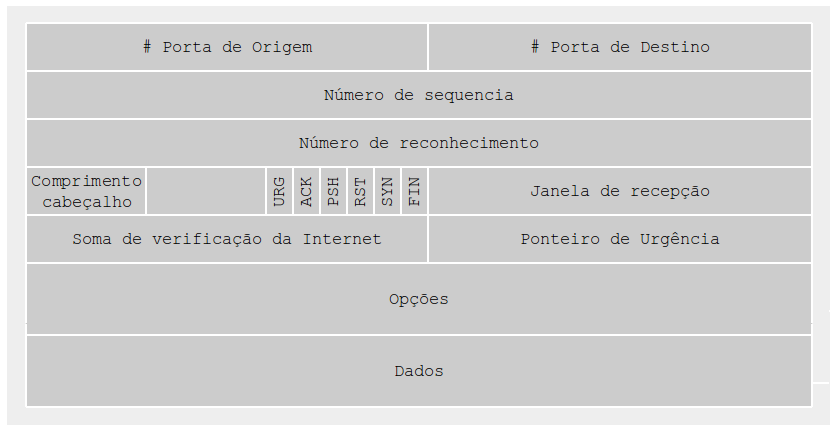
\includegraphics[width=\textwidth]{04-figuras/TCP.png}
    \caption{Estrutura da PDU do protocolo TCP}
    \label{fig:TCP}
    \fonte{\cite{KUROSE}}
\end{figure}

O mesmo autor declara que o protocolo UDP \cite{RFC768}, entretanto, faz o mínimo necessário para a entrega de dados de uma aplicação à outra, este adiciona ao IP apenas informações básicas para o encapsulamento da PDU em um segmento. É possível reparar a diferença quanto a simplicidade da estrutura do segmento do protocolo UDP, apresentado na Figura \ref{fig:UDP}, em comparação com a estrutura do segmento do protocolo TCP, mostrado na Figura \ref{fig:TCP}.

\begin{figure}
	\centering
    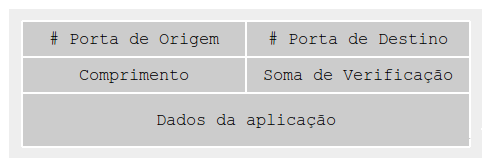
\includegraphics[width=0.75\textwidth]{04-figuras/UDP.png}
    \caption{Estrutura da PDU do protocolo UDP}
    \label{fig:UDP}
    \fonte{\cite{KUROSE}}
\end{figure}

As diferenças ressaltadas entre os protocolos TCP e UDP os tornam desejáveis para diferentes objetivos. Para conexões que são capazes de suportar perda de dados, como telefonia por Internet, ou necessitam de velocidade, como o protocolo DNS, é preferível a utilização do protocolo UDP. Já para os serviços que não suportam perdas e necessitam de confiabilidade, como HTTP, FTP e SMTP, o protocolo TCP é necessário.

Além dos protocolos citados, que são os mais conhecidos, \citeonline{FOR} citam outro protocolo pertencente a esta camada, o SCTP (\textit{Stream Control Transmission Protocol}), definido no RFC 4960 \cite{RFC4960}, que combina os melhores recursos dos protocolos TCP e UDP, assim ele provê um serviço confiável e orientado à mensagem.


\subsection{Rede}

Esta camada, também é chamada de internet (minúsculo para referenciar uma conexão de redes genérica), recebe o segmento enviado pela camada superior, de Transporte, juntamente com uma identificação do host para qual deve ser enviado este pacote, que então é encapsulado em um datagrama IP (Figura \ref{fig:IP}) e enviado para rede \cite{COMER}.Todos os pacotes transportados pela rede devem possuir o endereço de destino completo, número IP, pois estes serão independentemente transportados. 

\begin{figure}[H]
	\centering
    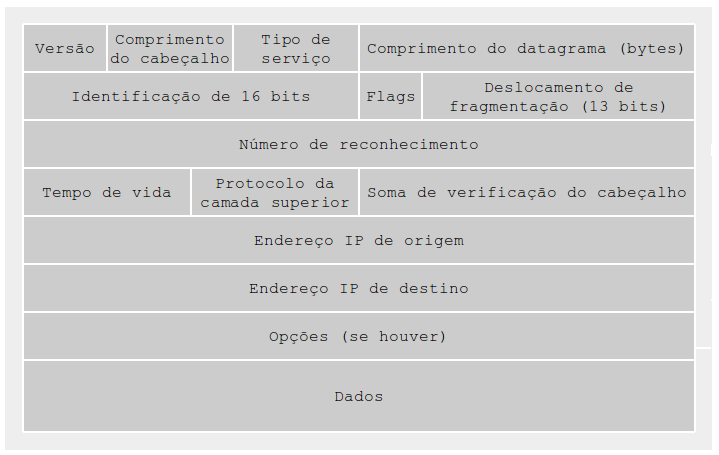
\includegraphics[width=\textwidth]{04-figuras/IPV4.png}
    \caption{Estrutura do datagrama IP}
    \label{fig:IP}
    \fonte{\cite{KUROSE}}
\end{figure}

O protocolo que define como a entrega desses pacotes deve ser feita é chamado de \textit{Internet Protocol}, o IP. O tipo de serviço oferecido pelo IP é chamado de serviço de melhor esforço, o que de acordo com \citeonline{KUROSE} não garante temporização preservada entre pacotes, recebimento destes em ordem no destinatário e nem garantia da entrega final. 

Sendo assim, a principal função desta camada, de acordo com \citeonline{TANENBAUM}, é o rotear pacotes da maquina origem para a máquina destino. Para isso são utilizados roteadores, que encaminham os pacotes recebido para o enlace de saída apropriado.


\subsection{Enlace}

De acordo com \citeonline{TANENBAUM} esta camada é mais propriamente definida como uma interface entre os hosts e os enlaces de transmissão (canais de comunicação que conectam nós adjacentes, sendo que nós refere-se à qualquer tipo de dispositivo que rode um protocolo da camada de enlace). Ela define o que os enlaces devem fazer para cumprir os requisitos de interconexão com o serviço não orientado a conexão oferecido pela camada superior, o IP.

\citeonline{KUROSE} definem dois tipos de enlaces: o primeiro tipo, de difusão (\textit{broadcast}) múltiplos hospedeiros são conectados em um só canal de comunicação (para que esta lógica seja possível é necessário um protocolo de acesso ao meio), os segundo tipo é o enlace de comunicação ponto-a-ponto, um único remetente e um único receptor em cad\texttt{\texttt{}}a extremidade do enlace.

Os pacotes de dados nesta camada são chamados de quadros, os quais são enviados pela rede em um fluxo de bits correspondentes. É necessário, então, lidar com erros de transmissão e regular o fluxo de dados para minimizar perdas. O padrão de transmissão de dados mais comumente utilizado é o Ethernet para redes locais fisicamente conectadas, também conhecido com IEEE 802.3.

Outro importante protocolo desta camada é protocolo ARP (\textit{Adress Resolution Protocol}), RFC 826 \cite{RFC826}, ele é responsável por obter o endereço físico, tamb\'em chamado endereço MAC (\textit{Media Access Control}), a partir do endereço passado pela camada de Rede acima, o endereço IP, permitindo assim a transmiss\~ao do quadro para seu destino.

\section{Aplicações}

Na própria Internet está disponível inúmeras aplicações que têm como foco redes e protocolos. Sobressaem-se simuladores de redes devido á sua funcionalidade tanto comercial quanto didática. Softwares com este objetivo são comercialmente interessantes para grandes empresas, pois possibilitam projetar e testar uma rede quanto ao seu desempenho, fluxo de dados, possíveis gargalos, perda de informações, segurança e etc., sem a necessidade de montar uma laboratório de testes, por exemplo, ou criar uma rede sem planejamento a qual pode vir a apresentar inúmeros problemas (como os já citados), opções estas muito mais dispendiosas.

Três destes simuladores são mais conhecidos: o \textit{Network Simulator}\footnote{https://www.nsnam.org/} (NS3) um software aberto, voltado especialmente para pesquisa e uso educacional; o \textit{Cisco Packet Tracer}\footnote{http://www.packettracernetwork.com/} desenvolvido pela Cisco\textregistered, que permite a simulação de uma rede utilizando diferentes equipamentos da marca (seu objetivo didático inclui o treinamento para certificação oferecidas pela própria empresa); e o GNS3\footnote{https://www.gns3.com/} que além do software de simulação mantêm uma comunidade online para discussões e troca de ideias para seus usuários. 

Além dos simuladores existem outras aplicações interessantes, conhecidas como \textit{sniffers}, que interceptam e analisam o tráfego de rede, ou seja os pacotes enviados e recebidos em uma conexão. O mais conhecido deles é o \textit{Wireshark}\footnote{https://www.wireshark.org/}, um analisador de protocolos utilizado para navegação interativa do tráfego de rede em tempo real.

